\chapter{Magnetosensory Power Devices}
\label{ch:Magnetosensory Power Devices}

% **************************** Define Graphics Path **************************
\ifpdf
    \graphicspath{{Chapter4/Figs/Raster/}{Chapter4/Figs/PDF/}{Chapter4/Figs/}}
\else
    \graphicspath{{Chapter4/Figs/Vector/}{Chapter4/Figs/}}
\fi

\section{Background and motivation}
\label{sec:Background and motivation}
Biological \index{Magnetosensory power MEMS devices (MPD)} studies have suggested that a variety of animals have the ability to perceive the geomagnetic field, including insects \cite{dreyer2018earth}, amphibians \cite{fischer2001evidence}, reptiles \cite{diego2017spontaneous}, fish \cite{naisbett2020magnetoreception}, and birds \cite{ossenkopp1978bird}. Migratory birds, for instance, have been suggested to not only orient themselves by sensing the inclination of the field \cite{ritz2000model}, but also may deduce their location by discerning minute local variations in the geomagnetic field \cite{kishkinev2015eurasian,mouritsen2005magnetoreception}. Driven by the ongoing rapid advance of artificial intelligence (AI), neuroscience, and bionics, the development of bionic \index{Bionic} smart devices has made significant progress, such as the bionic eye \cite{ong2012bionic}, artificial synapse network \cite{zhu2014artificial}, bionic artificial nerve \cite{liao2020bioinspired}, bionic skins \cite{cao2019self}, etc. The biophysical mechanisms that underlie magnetoreception in nature would be an appealing source from which inspiration can be drawn to develop magnetosensory power devices for \index{Interactive electronic} interactive electronics \cite{canon2018electronic,makushko2021flexible}. Traditional magnetic sensors have been proposed as a way to interact with objects in a touchless manner and move beyond conventional tactile interactions. Such sensors have been applied to magnetosensitive e-skins \cite{canon2018magnetosensitive} and wearable magnetic sensors \cite{melzer2015wearable}. However, due to their discrete design and low output power density, these magnetic sensors can usually only be used as sensing devices, and therefore require bulky analog amplifiers as actuators, which are difficult to be applied as interactive electronic \index{Interactive electronic} systems with high integration and high power density. The demand for operating power of new intelligent bionic devices has promoted the cross-study of magnetosensory power devices, thereby realizing the integrated interactive electronic system of non-contact sensing and execution. \index{Magnetosensory power MEMS devices (MPD)}

As the important representative of the power semiconductor materials, III-nitride \index{Nitride} compound semiconductor materials have important application prospects in the fields of power electronics \cite{ueda2019gan}, due to the high carrier density, high electron \index{Electron mobility} mobility, and wide bandgap. More significantly, III-nitrides show obvious spontaneous \index{Spontaneous polarization} and \index{Piezoelectric!polarization} piezoelectric polarization, which accounts well for the modulation \index{Modulation} of the energy band \index{Energy band} profile and two-dimensional electron gas (2DEG) concentration \index{Two-dimensional electron gas (2DEG)} in the heterojunction \cite{ambacher2000two,jena2010polarization,yu1999spontaneous}. Based on coupling effects of semiconductor characteristics and piezoelectric characteristics, the piezotronics \index{Piezotronics} effect can be observed in III-nitrides \cite{pan2019piezotronics,wang2018piezotronics,sha2019iii}, and it opens a window to strain-regulated nanowires \cite{wang2016piezotronic,wang2006piezoelectric}, LEDs \cite{huang2016piezo,liu2020piezo,guo2021enhanced}, and HEMTs \cite{jiang2017piezotronic,wang2016piezotronic,hua2021piezotronics}, especially in the artificial intelligence devices \cite{hua2021piezotronics,johnsen2005physics}.

Here, we present a bioinspired magnetosensory power device (MPD) that can demonstrate large output power \index{Output!power} control with the emulation of magnetoreception in nature. The MPD is based on a \index{Cantilever} cantilever-structured AlGaN/AlN/GaN HEMT \index{HEMT} device integrated with a high magnetic \index{Magnetic!thin film} film \ce{(Fe90Co10)78Si12B10}. The cantilever \index{Cantilever} structure of the MPD is an ingenious design that can help to amplify the sensitivity of the output current/power in response to the change of external magnetic \index{Magnetic!field} field. It is observed that MPD has a sensitive magnetic field-power modulation response. Meanwhile, the gate voltage \index{Voltage!gate voltage} of the MPD can finally control the operating point of the \index{Output!power} output power, indicating the robust and programmable characteristics of the MPD. According to the experiment and simulation results, the modulation \index{Modulation} relationship between the output power of the MPD and the external \index{Magnetic!field} magnetic field is quasi-linear, showing excellent output power control characteristics with magnetic field. This work not only provides bioinspired device insights into the mechanism of magnetoreception, but also promotes the development of high power interactive electronic and AI smart devices. It can be expected that MPD will have excellent application prospects in interactive electronics, artificial intelligence, and robotics.

\begin{figure}[H] 
\centering    
\includegraphics[width=0.9\textwidth]{ch4_1}
\caption[Illustration of the magnetosensory power device (MPD) inspired by magnetoreception in birds]{Illustration of the magnetosensory power device (MPD) inspired by magnetoreception in birds. (a) Schematic diagram of the birds’ navigation and orientation through the geomagnetic field. (b) Schematic diagram of the MPD.}
\label{fig:4.1}
\end{figure}

The \index{Magnetosensory power MEMS devices (MPD)} magnetoreception \index{Magnetoreception} in nature has fascinated scientists due to its unique biological and bionic \index{Bionic} characteristics. For example, pigeons can locate themselves and determine directions by sensing the geomagnetic field. \autoref{fig:4.1} illustrates the magnetoreception in birds and bioinspired magnetosensory power device (MPD). The external magnetic field applied to the MPD can mimic the mechanism of magnetoreception to control the output current and power with the external magnetic field stimulus. The geomagnetic sense of the biological model of birds is schematically displayed in \autoref{fig:4.1}a. Under the action of geomagnetic field, the current signals of neurons between synapses in birds can be significantly modulated for location and orientation \cite{zhang2020strain}. 


\section{Design and preparation}
\label{sec:Design and preparation}

\subsection{Device structure and characterization}
\label{sec:Device structure and characterization}

\autoref{fig:4.1}b shows \index{Magnetosensory power MEMS devices (MPD)} the schematic diagram of the cantilever-based \index{Cantilever} magnetosensory power device MPD. The designed MPD is based on the cantilever-structured \index{HEMT} AlGaN/GaN high-electron-mobility transistor (HEMT), in which a magnetic thin film \index{Magnetic!thin film} \ce{(Fe90Co10)78Si12B10} is deposited on the front end of the cantilever. The enlarged part is the schematic cross-section of the AlGaN/GaN HEMT, where from top to bottom are AlGaN, AlN, GaN, and Si substrate. The thicknesses of AlGaN, AlN, and GaN layers are 30 \unit{\nm}, 1 \unit{\nm}, and 4.3 \unit{\um}, respectively, and the active region of MPD is \numproduct{34 x 34} \unit{\square\um}. The structural parameters of HEMT and MPD are detailed in \autoref{tab:4.1}. It can be clearly seen that MPD has a more complex cantilever structure with a magnetic film deposited compared to traditional HEMT on AlGaN/AlN/GaN epitaxial wafers. When the MPD senses an external \index{Magnetic!field} magnetic field, the magnetic \index{Magnetic!force} force on the magnetic film at the front end of the cantilever \index{Cantilever} will cause bending strain on the active region of the MPD. Based on the piezotronics \index{Piezotronics} effect, the bending strain of the active region \index{Active region} will induce piezoelectric \index{Piezoelectric!polarization charge} polarization charges in the AlGaN, AlN, and GaN layers, thereby adjusting the AlGaN/AlN/GaN heterojunction \index{AlGaN/AlN/GaN heterojunction} energy band \index{Energy band} and 2DEG \index{Two-dimensional electron gas (2DEG)} concentration, and finally modulating the output current \index{Output!current} and power \index{Output!power} of MPD. Therefore, the MPD manifests effective power modulation characteristics under the stimulation of external magnetic field, realizing high-power interactive electronics with non-contact sensing and control.

\begin{table}[H]
\renewcommand\arraystretch{1.5}
\centering
\caption[Structural parameters of HEMT and MPD]{Structural parameters of HEMT and MPD}
\begin{tabular}{ccccc}
\hline \hline
MPD design    & Material            & Length (\unit{\um}) & Width (\unit{\um}) & Thickness (\unit{\nm}) \\ \hline \hline
Cantilever    & GaN                 & 350         & 60         & 4300        \\
Magnetic film & \ce{(Fe90Co10)78Si12B10} & 175         & 60         & 500         \\
HEMT          & AlGaN/AlN/GaN       & 34          & 34         & 30/1/4300  \\ \hline \hline
\end{tabular}
\label{tab:4.1}
\end{table}

The \index{Magnetosensory power MEMS devices (MPD)} fabrication \index{Fabrication process} process of MPD is shown in \autoref{fig:4.2}a. We first prepare the HEMT device on the AlGaN/AlN/GaN epitaxial wafer, then deposit a magnetic film \ce{(Fe90Co10)78Si12B10} in the front end of the active \index{Active region} region, and finally released the cantilever \index{Cantilever} structure of GaN. To fabricate the GaN-based cantilever, we perform a fully dry etching process by using inductively coupled plasma etching (ICP) \cite{yang2015influence}. We first remove GaN layer by anisotropic etching \index{Etching!anisotropic etching} of GaN, and the cantilever structure is laterally released by isotropic etching \index{Etching!isotropic etching} of Si. The dry etching \index{Etching!dry etching} process has its own unique advantages, such as precise controllability, patterning, and good repeatability. By simply adjusting the etching time and recipe, we can manufacture the cantilever-based structure MPD under precise control, which is of great significance for the integrated MEMS application of MPD. The main fabrication process can be briefly divided into four steps shown in \autoref{fig:4.2}a. Step 1: (a1) Initial Si-based AlGaN/AlN/GaN epitaxial layer; Step 2: (a2) The mesa isolation \index{Mesa isolation} etching of AlGaN, AlN, and GaN by \index{Inductively coupled plasma (ICP)} ICP; Step 3: (a3) Electron beam deposition to prepare Ohmic contact and Schottky \index{Contact!Schottky contact} contact \index{Contact!Ohmic contact} electrodes, as well as magnetic \index{Magnetic!thin film} film; Step 4: (a4) The released cantilever by ICP. The device fabrication process is also detailed in the \autoref{sec:Fabrication processes}. The scanning electron microscopy (SEM) \index{Scanning electron microscopy (SEM)} image and the inset optical picture taken by CCD camera of \autoref{fig:4.2}b clearly displays the manufactured MPD, from which the complete cantilever \index{Cantilever} structure and the HEMT \index{HEMT} device can be easily observed. The active region is located at the junction between the end of the cantilever \index{Cantilever} and \index{Substrate} the substrate, and therefore bears the greatest bending strain under the action of external stress, which induces piezoelectric polarization charges \index{Piezoelectric!polarization charge} in the AlGaN/AlN/GaN interface and modulates the output power of the MPD. The high-resolution TEM image acquired from the AlGaN/AlN/GaN hetero-stacks is displayed in \autoref{fig:4.2}c. It is clearly shown that the interface \index{Interface} atoms of AlGaN/AlN and AlN/GaN are uniform and sharp without apparent boundary defects or dislocations, and the layers of GaN, AlN, and AlGaN can be easily identified. 

\begin{figure}[H] 
\centering    
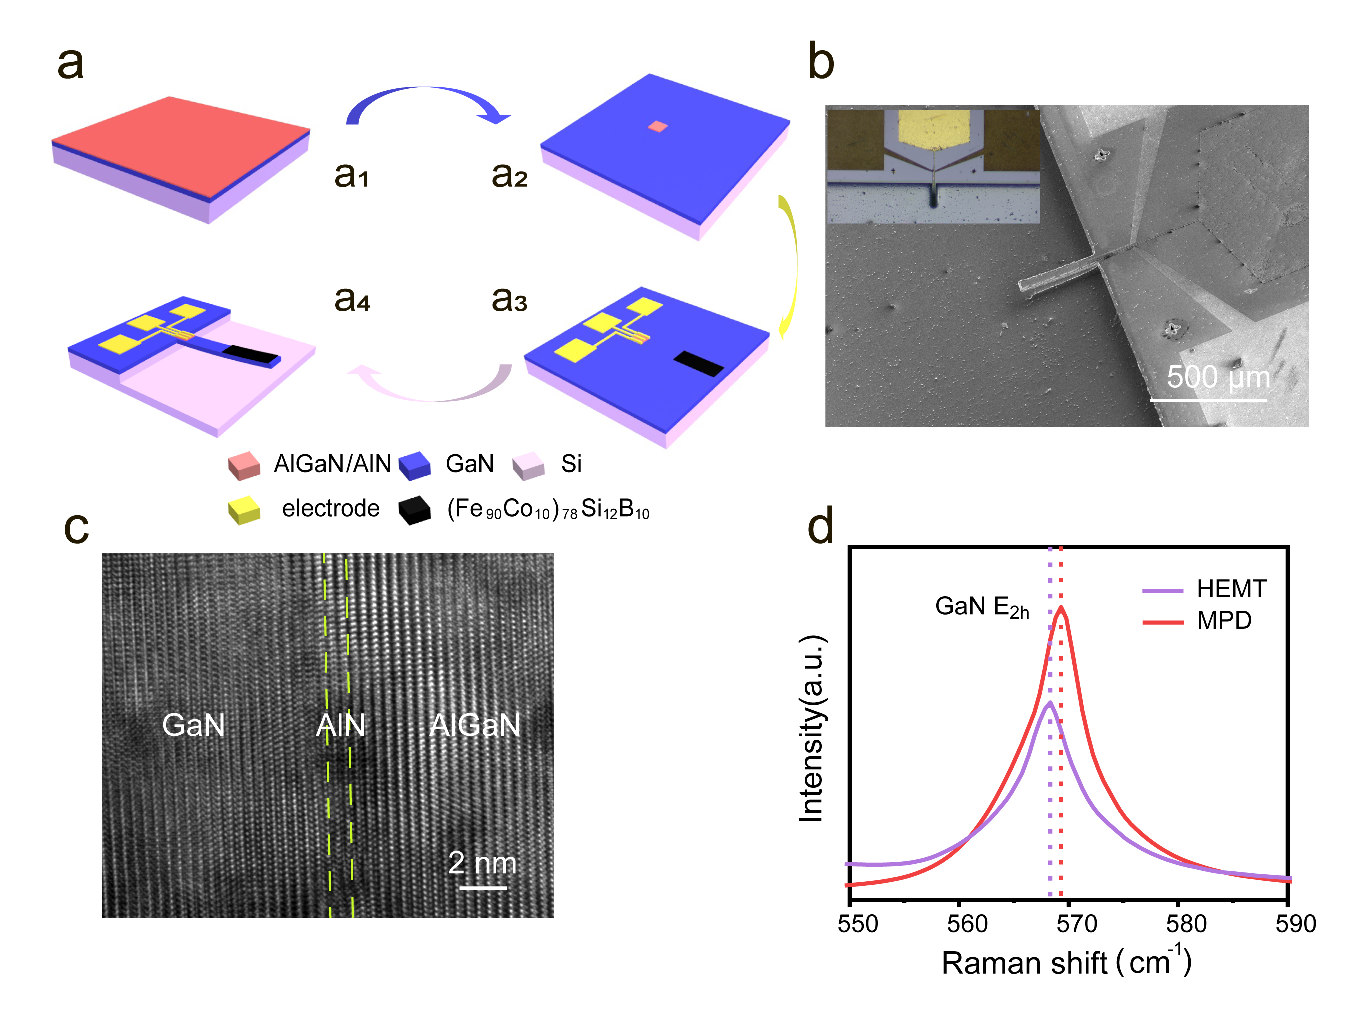
\includegraphics[width=0.9\textwidth]{ch4_2}
\caption[The fabrication process and characterization of MPD]{The fabrication process and characterization of MPD. (a) The fabrication flow chart. (b) The SEM and CCD image. (c) The TEM image acquired from the AlGaN/AlN/GaN hetero-stacks. (d) The micro-Raman spectra of the AlGaN/AlN/GaN heterostructures before (HEMT) and after (MPD) dry-etching.}
\label{fig:4.2}
\end{figure}

The \index{Magnetosensory power MEMS devices (MPD)} Raman spectroscopy \index{Raman!spectroscopy} tests on both HEMT \index{HEMT} and MPD at room temperature have been performed to reveal the influence of the ICP dry etching \index{Etching!dry etching} process on the electrical performance of MPD, as shown in \autoref{fig:4.2}d. The MPD exhibits that the $E_{2h}$ phonon mode of GaN shows a blue shift from 568.31 \unit{\per\cm} to 569.33 \unit{\per\cm} compared with the HEMT, which reveals that the dry etching process releases the silicon substrate and relaxes the tensile strain of the GaN layer \cite{yang2015influence,wang2016piezotronic}. The alleviation of the tensile strain of the GaN layer will partially weaken the piezoelectric polarization effect of the GaN layer, thereby reducing the 2DEG concentration \index{Two-dimensional electron gas (2DEG)} in the \index{AlGaN/AlN/GaN heterojunction} AlGaN/AlN/GaN heterojunction. The relationship between the biaxial stress \index{Biaxial stress model} and the shift of the Raman phonon frequency \index{Raman!phonon frequency} is shown in \autoref{eq:4.1}. 
\begin{equation}
\sigma _{a}=\frac{\Delta \omega}{K_{\mathrm{RS}}^{\mathrm{E} 2(h i g h)}}
\label{eq:4.1}
\end{equation}
where $\sigma _{a}$ is the in-plane biaxial stress, $\Delta \omega$ is the shift of the Raman phonon frequency, and $K_{\mathrm{RS}}^{\mathrm{E} 2(h i g h)}$ is the Raman biaxial stress \index{Raman!biaxial stress conversion factor} conversion factor. We can obtain that the tensile stress of the GaN epitaxial layer is reduced by 352 \unit{\MPa} compared with that on the Si substrate \cite{choi2013analysis}. In addition, lattice defects have also been introduced during the dry etching process, which reduces the electrical performance of MPD to a certain extent \cite{ladroue2010deep,pearton2000review,huang2004inductively}. Therefore, ICP \index{Inductively coupled plasma (ICP)} dry etching \index{Etching!dry etching} will inevitably degrade the performance of MPD during the preparation of the \index{Cantilever} cantilever. Comparing the performance of MPD and HEMT in \autoref{fig:4.4}, it can be concluded that due to the ICP etching process in the cantilever fabrication process, the electrical properties of MPD are degraded to a certain extent compared to HEMT devices. Literature studies have shown that this performance \index{Degradation} degradation is unavoidable in the process of fabricating cantilever structures using the ICP process, but we have improved the performance degradation during cantilever fabrication through process optimization. Compared to the electrical properties of SPD \index{Strain-controlled power MEMS devices (SPD)} in \autoref{ch:Strain-controlled power devices}, the electrical performance of MPD has been greatly improved, which is detailed in the fabrication process subsection.

\autoref{fig:4.3}a illustrates \index{Magnetosensory power MEMS devices (MPD)} the EDX \index{Energy-dispersive X-ray spectroscopy (EDX)} line profiles for the element of Ga (red), Al (green), and N (purple) and energy-dispersive X-ray spectroscopy (EDS) element mapping including Ga, Al, and N acquired from the AlGaN/AlN/GaN hetero-stacks, which evidently displays the AlGaN/AlN/GaN heterostructure and confirms the chemical element composition. The high-resolution TEM \index{Transmission electron microscopy (TEM)} image acquired from the AlGaN/AlN/GaN hetero-stacks is displayed in \autoref{fig:4.3}b. It is clearly shown that the interface atoms of AlGaN/AlN and AlN/GaN are uniform and sharp without apparent boundary defects or dislocations, and the layers of GaN, AlN, and AlGaN can be easily identified.

\begin{figure}[H] 
\centering    
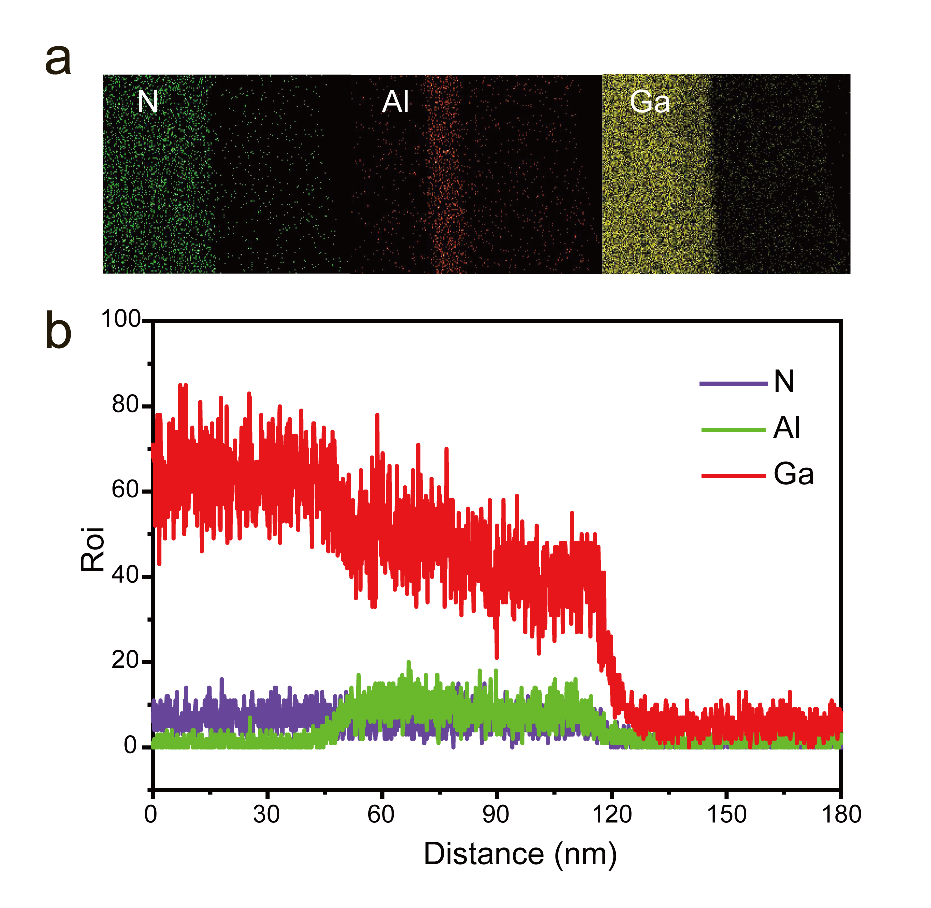
\includegraphics[width=0.7\textwidth]{ch4_3}
\caption[The EDX line profiles for the element of Ga (red), Al (green), and N (purple) and energy-dispersive X-ray spectroscopy (EDS) element mapping including Ga, Al, and N acquired from the AlGaN/AlN/GaN hetero-stacks]{The EDX line profiles for the element of Ga (red), Al (green), and N (purple) and energy-dispersive X-ray spectroscopy (EDS) element mapping including Ga, Al, and N acquired from the AlGaN/AlN/GaN hetero-stacks.}
\label{fig:4.3}
\end{figure}

\subsection{Fabrication processes}
\label{sec:Fabrication processes}

The \index{Magnetosensory power MEMS devices (MPD)} MPD was fabricated with III-Nitride \index{Nitride} epitaxial layers \index{Epitaxial!layer} by metal-organic chemical vapor deposition (MOCVD) \index{MOCVD} on Si substrate ($111$). The epitaxial layer structure consists of AlGaN (30 \unit{\nm}, 30$\%$ Al) / AlN (1 \unit{\nm}) / GaN (4.3 \unit{\um}) / AlGaN buffer layer / Si substrate. The mesa was etched using an inductively coupled plasma etching system (ICP, SENTECH SI 500) etch process based on \ce{BCl3}/\ce{Cl2}/\ce{Ar}. In order to form the ohmic \index{Contact!Schottky contact} contact and Schottky \index{Contact!Ohmic contact} contact, Ti/Al/Ni/Au (20 \unit{\nm} / 120 \unit{\nm} / 45 \unit{\nm} / 55 \unit{\nm}) metal stack deposition was evaporated using an electron beam evaporation \index{Deposition!electron beam evaporation} system (Denton Vacuum Explore 14) and annealed at \SI{900}{\degreeCelsius} in \ce{N2} environment for 30 \unit{\s} using a rapid thermal processing \index{Rapid thermal!processing (RTP)} system (LABSYS RTP-1200), and Ni/Au (80 \unit{\nm} / 50 \unit{\nm}) was evaporated for gate metallization respectively. Then the magnetic film \ce{(Fe90Co10)78Si12B10} (500 \unit{\nm}) was deposited by magnetron sputtering \index{Deposition!magnetron sputtering} (Denton Discovery 635). Finally, the ICP-based dry etching was performed by combing the \index{Etching!isotropic etching} anisotropic/isotropic etching \index{Etching!anisotropic etching} to fabricate the cantilever \index{Cantilever} using an inductively coupled plasma etching \index{Inductively coupled plasma (ICP)} system (ICP, SENTECH SI 500). The main steps of the etching process of the cantilever \index{Cantilever} structure based on ICP dry etching \index{Etching!dry etching} are as follows: Step 1: anisotropic etching of GaN. The photoresist patterned GaN thin film (thickness: 5 \unit{\um}) is completely etched with the anisotropic etching recipe (\ce{BCl3}/\ce{Cl2}/\ce{Ar}: 10/32/5 sccm; Power: \SI{550}{\watt}; Process time: 30 \unit{\minute}). Step 2: isotropic etching of Si. The cantilever \index{Cantilever} structure is fabricated with the isotropic etching recipe (\ce{SF6}/\ce{O2}/\ce{Ar}: 30/5/10 sccm; Power: \SI{800}{\watt}; Process time: 25 \unit{\minute}). The manufactured cantilever \index{Cantilever} had dimensions of \numproduct{350 x 60 x 5} \unit{\cubic\um}, with the embedded HEMT had a mesa dimension of \numproduct{34 x 34} \unit{\square\um} and a gate length of 5 \unit{\um}.

It \index{Magnetosensory power MEMS devices (MPD)} is worth noting that a significant performance degradation \index{Degradation} before and after cantilever \index{Cantilever} etching was observed during the preparation of SPD \index{Strain-controlled power MEMS devices (SPD)} in \autoref{ch:Strain-controlled power devices}, which is because the long-term ICP etching introduces a large number of lattice \index{Lattice!defects} defects. As a result, the electrical conductivity and electrode contact performance of the SPD is greatly reduced. So if the active area of ​​the device can be more effectively protected during prolonged ICP etching, the electrical performance of the device will be significantly improved. In the process of preparing the cantilever \index{Cantilever} structure of MPD in this study, the thickness of the photoresist as the anti-etching mask layer is significantly increased by applying multiple layers of \index{Photoresist} positive photoresist. The UV exposure and development parameters of the photoresist under the corresponding thickness have been explored through the experimental process, therefore a mask layer with high etching resistance with a complete pattern  has been successfully prepared. The experimental results show that the high etch-resistance mask layer composed of multi-layer photoresist effectively protects the active area of ​​the device, and the performance degradation of MPD before and after cantilever \index{Cantilever} etching is greatly improved. Compared with unetched HEMT, when $V_{gs}$ = 0 \unit{V} and $V_{ds}$ = 10 \unit{V}, the saturated output current of MPD is only reduced by 67 \unit{\mA\per\mm}, while the saturated output current of SPD \index{Strain-controlled power MEMS devices (SPD)} under the same conditions is reduced by 250 \unit{\mA\per\mm}. Therefore, by applying photoresist in multiple layers, we have successfully improved the fabrication process \index{Fabrication process} of cantilever \index{Cantilever} MEMS devices based on \index{AlGaN/AlN/GaN heterojunction} AlGaN/AlN/GaN heterojunctions, and explored a new process method for the preparation of higher performance cantilever \index{Cantilever} MEMS devices in the future.

\section{Device performance}
\label{sec:Device performance}

\subsection{Electrical performance}
\label{sec:Electrical performance}

The \index{Magnetosensory power MEMS devices (MPD)} electrical \index{Current!drain current} characteristics of HEMT (before the dry-etching for the cantilever \index{Cantilever} structure) and manufactured MPD are shown in \autoref{fig:4.4}. Based on the good electrical contact performance, the output characteristics ($I_{ds}$-$V_{ds}$) of both HEMT \index{HEMT} and MPD have excellent gate control capabilities, as shown in \autoref{fig:4.4}a,c, respectively. It is clearly shown that the output current shows good linearity at low source-drain \index{Voltage!source-drain voltage} bias ($V_{ds}$) voltage, and then as the bias voltage further increases, the output current reaches saturation. Both HEMT \index{HEMT} and MPD can achieve stable large output current \index{Output!current} above 200 \unit{\mA\per\mm} in the saturation region, and can be effectively controlled at various gate voltage \index{Voltage!gate voltage} ($V_{gs}$) from -7 \unit{\V} to 1 \unit{\V}. Compared with HEMT, the saturated output current of MPD under the source-drain bias voltage of 10 \unit{\V} drops from 264 \unit{\mA\per\mm} to 197 \unit{\mA\per\mm}. Furthermore, we measure the transfer ($I_{ds}$-$V_{gs}$) characteristics of the HEMT and the MPD at $V_{ds}$ = 10 \unit{\V}, as shown in \autoref{fig:4.4}b,d, respectively. The maximum transconductance \index{Transconductance} ($g_{m, max}$) of HEMT is 42.4 \unit{\mA\per\mm} (\autoref{fig:4.4}b), while the value for the MPD reduces to 32.9 \unit{\mA\per\mm} (\autoref{fig:4.4}d). The transconductance performance of MPD is also slightly lower than HEMT. The reduction in the output current and transconductance of the MPD can be attributed to the dry etching \index{Etching!dry etching} process, which inevitably leads to stress release and \index{Current!drain current} lattice defects \index{Lattice!defects} in the GaN layer. 

\begin{figure}[H] 
\centering    
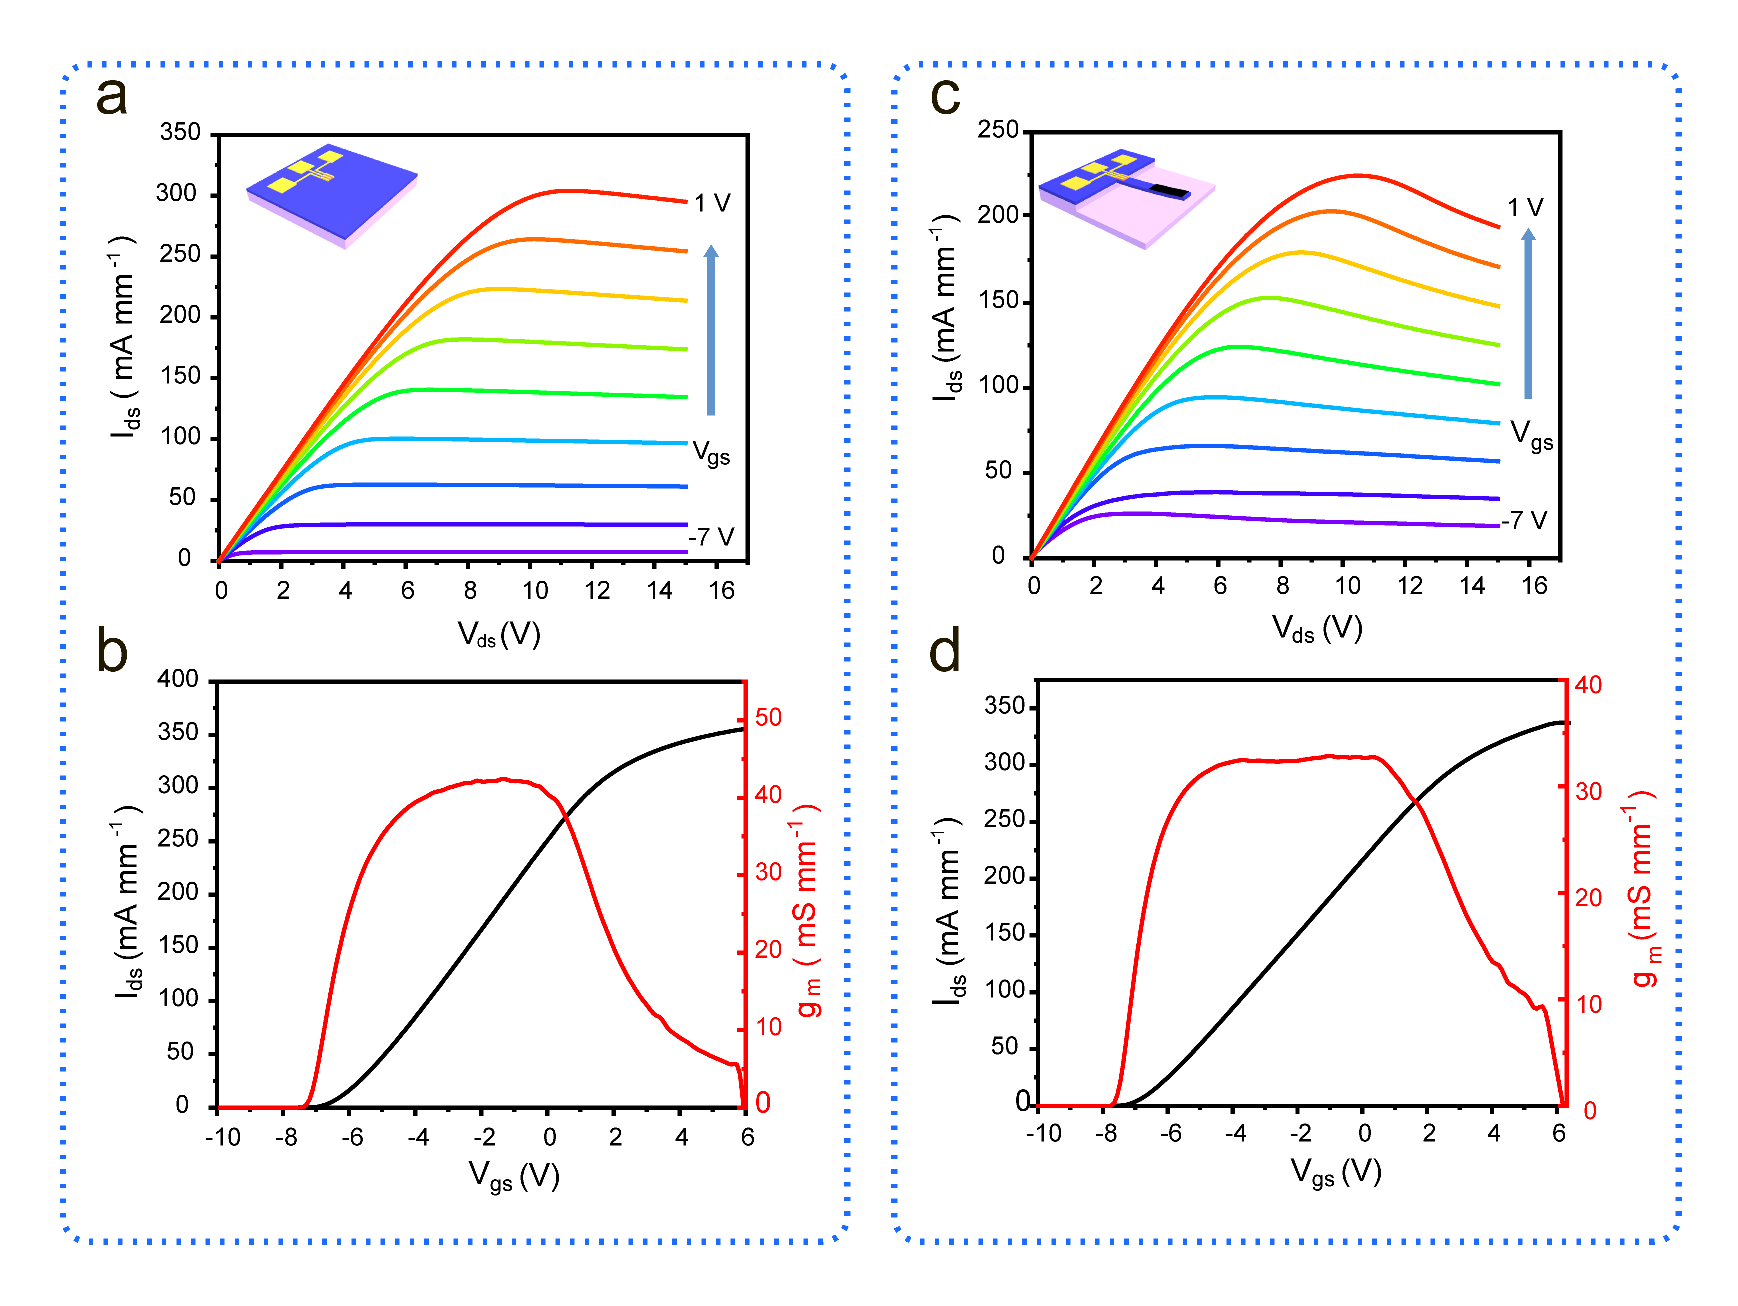
\includegraphics[width=0.9\textwidth]{ch4_4}
\caption[Electrical characteristics of the HEMT (before etching) and the as-fabricated MPD]{Electrical characteristics of the HEMT (before etching) and the as-fabricated MPD. Output ($I_{ds}$-$V_{ds}$) characteristics of the (a) HEMT and (c) MPD. Transfer ($I_{ds}$-$V_{gs}$) characteristics of the (b) HEMT and (d) MPD measured.}
\label{fig:4.4}
\end{figure}

Both \index{Magnetosensory power MEMS devices (MPD)} HEMT \index{Cantilever} and MPD exhibit good Schottky contacts \index{Contact!Schottky contact} on the gate and Ohmic contacts \index{Contact!Ohmic contact} on the source and drain (\autoref{fig:4.5}a,b). However, the Schottky contact performance of MPD is slightly worse than that of HEMT, which is caused by the lattice defects introduced by the ICP process \cite{choi2003observation,cao2000schottky} and the enhanced self-heating effect after etching \cite{yang2011high,hajjiah2020effect,greco2017temperature}. It can be concluded that due to the dry etching process, the electrical performance of MPD is slightly lower than that of HEMT, but it still has excellent output characteristics and transfer characteristics. The leakage current characteristics of HEMT and MPD are shown in \autoref{fig:4.5}c,d, respectively. It is clearly shown that the ICP process does not significantly increase the leakage current \index{Current!leakage current} of the device. The SPD \index{Strain-controlled power MEMS devices (SPD)} maintains substantially the same leakage current characteristics \index{Current!drain current} as the HEMT.

\begin{figure}[H] 
\centering    
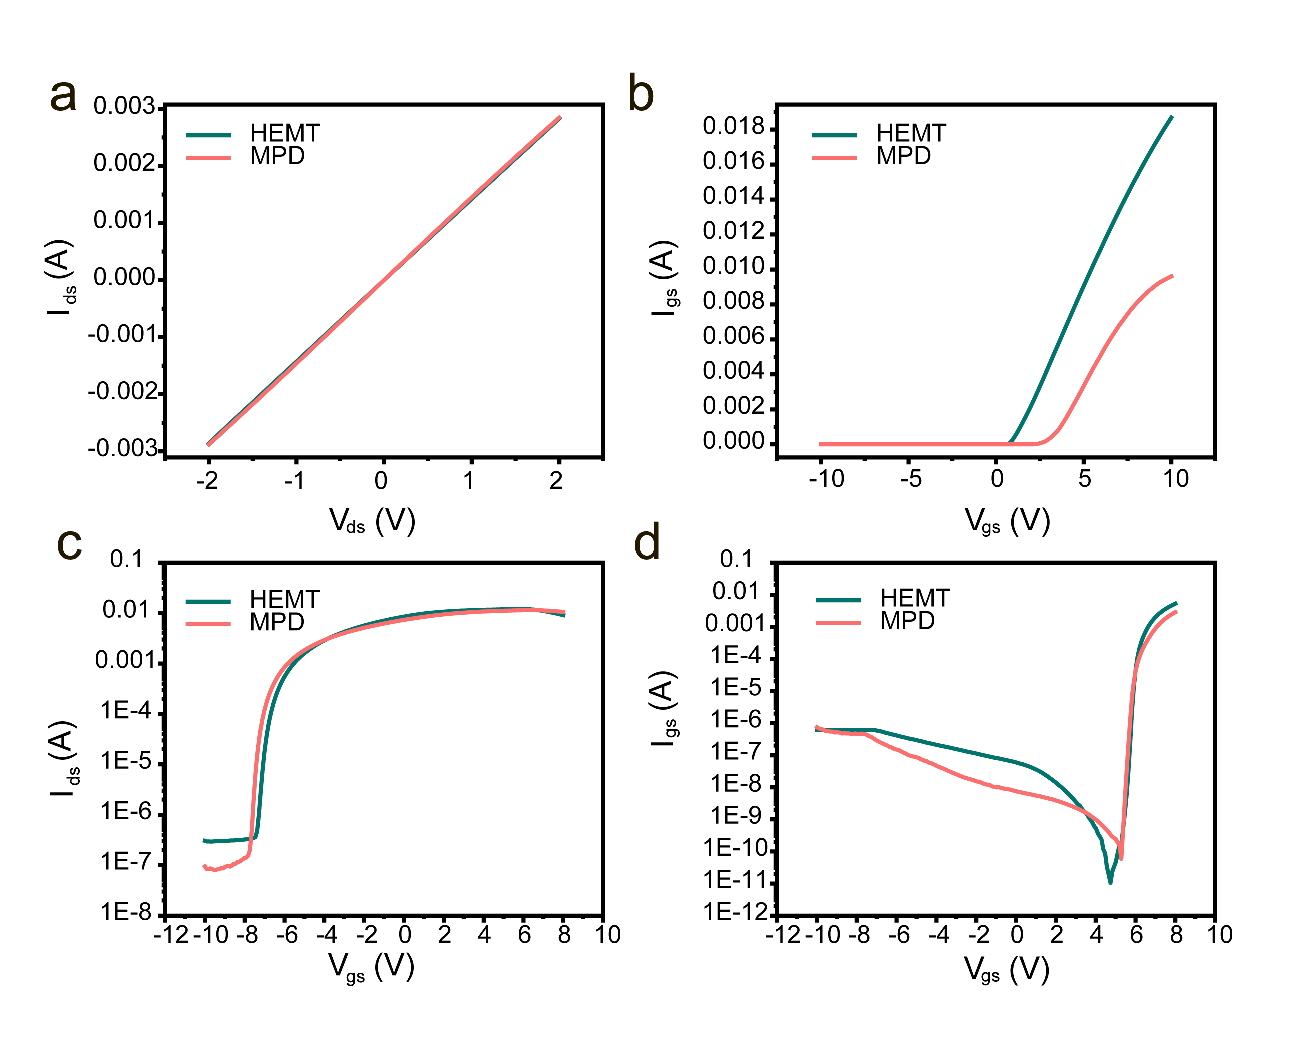
\includegraphics[width=0.9\textwidth]{ch4_5}
\caption[The contact and leakage characteristics of HEMT and MPD]{The contact and leakage current characteristics of HEMT and MPD (a) The source-drain Ohmic contact and (b) gate Schottky contact characteristics. (c) The $I_{ds}-V_{gs}$ characteristics and (d) gate leakage currents characteristics.}
\label{fig:4.5}
\end{figure}


\subsection{Magnetic field-power modulation performance}
\label{sec:Magnetic field-power modulation}

Different \index{Magnetosensory power MEMS devices (MPD)} magnetic fields \index{Magnetic!field} are applied to the MPD under various gate voltages \index{Voltage!gate voltage} to mimic \index{Magnetoreception} the magnetoreception. The modulation \index{Modulation} characteristics of the external magnetic field on the output current and power of the MPD are systematically discussed. In this study, we design an energized solenoid to generate a uniform controllable magnetic field, and in order to enhance the magnetic field inside the energized solenoid, we design a correspondingly sized iron core. According to the Biot-Savart law, the magnetic \index{Magnetic!field} field inside a long energized solenoid can be approximately regarded as a uniform magnetic field. By changing the current of the energized solenoid and calibrating with a magnetic field detector, the magnetic field acting on the MPD can be accurately controlled. We put the MPD inside the energized solenoid and change the input current of the solenoid to generate the magnetic fields of 0 \unit{\milli\tesla}, 100 \unit{\milli\tesla}, 200 \unit{\milli\tesla}, 300 \unit{\milli\tesla}, and 400 \unit{\milli\tesla}, respectively. The source-drain voltage \index{Voltage!source-drain voltage} $V_{ds}$ and the gate-source voltage \index{Voltage!gate-source voltage} $V_{gs}$ are used to measure the output characteristics and transfer characteristics of the MPD under different external magnetic fields.

\autoref{fig:4.6}a illustrates the strain \index{Strain} distribution of the MPD under an external magnetic field of 400 \unit{\milli\tesla}, which is simulated by COMSOL Multiphysics \index{Finite element analysis} and the magnetic force \index{Magnetic!force} on the MPD cantilever \index{Cantilever} is in the negative $z$ direction. It clearly shows that due to the design of the cantilever \index{Cantilever} structure, the active region \index{Active region} of the MPD bears the strain under the action of the magnetic field, thereby enhancing the piezotronics \index{Piezotronics} effect and increasing the modulation of the output power by the magnetic field. Figure 4b displays the output characteristics of the MPD under an external magnetic field of 200 \unit{\milli\tesla}, with the gate voltage $V_{gs}$ ranging from -5 \unit{\V} to 1 \unit{\V} at a step of 1 \unit{\V}. Under the same magnetic field, the modulation effect of the current density becomes more significant with the increase of $V_{gs}$, which means that the \index{Output!current} output current response to the external magnetic field is effectively modulated by the gate \index{Voltage!gate voltage} voltage. 

In \index{Magnetosensory power MEMS devices (MPD)} addition, the output \index{Current!drain current} current of the MPD can also be effectively modulated by an external magnetic field. \autoref{fig:4.6}c illustrates the output characteristics of MPD under various external magnetic fields when $V_{gs}$= -5 \unit{\V}. As the magnetic field increases, the output current density of the MPD increases in both the linear and saturation regions. At $V_{gs}$= -5 \unit{\V} and $V_{ds}$= 15 \unit{\V},

\begin{figure}[H] 
\centering    
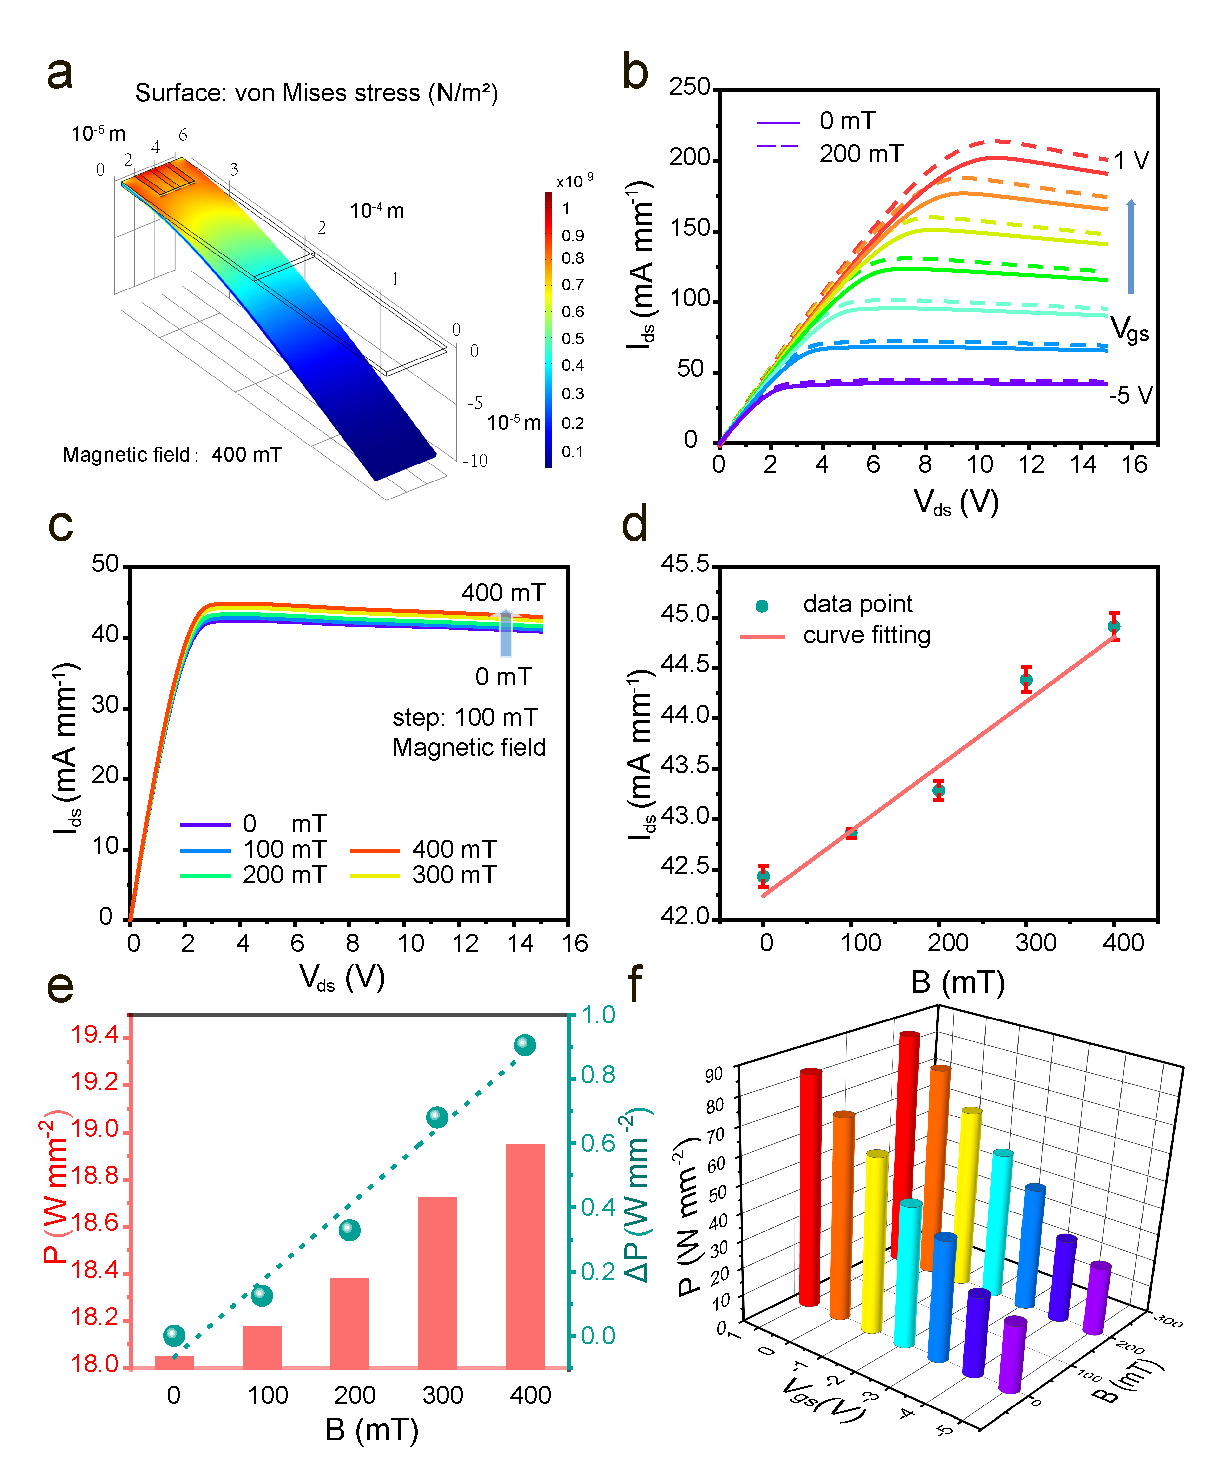
\includegraphics[width=0.9\textwidth]{ch4_6}
\caption[The magnetic field-power modulation characteristics of MPD]{The \index{Cantilever} magnetic field-power modulation characteristics of MPD. (a) The strain distribution under the magnetic field of 400 \unit{\milli\tesla}. (b) Output \index{Magnetosensory power MEMS devices (MPD)} characteristics under the magnetic field of 200 \unit{\milli\tesla}. (c) Output \index{Current!drain current} characteristics under the magnetic field with 0 $\sim$ 400 \unit{\milli\tesla} at $V_{gs}$= -5 \unit{\V}. (d) The curve fitting of the saturation output current in (c) under the magnetic field at $V_{ds}$= 15 \unit{\V}, $V_{gs}$= -5 \unit{\V}. (e) Output power density plots under the magnetic field with 0 $\sim$ 400 \unit{\milli\tesla} at $V_{gs}$= −5 \unit{\V}. (f) 3D plots illustrating the relationship between the output power density and the magnetic field or gate voltage.}
\label{fig:4.6}
\end{figure}

\noindent when the magnetic field increases from 0 to 400 \unit{\milli\tesla}, the saturation current of the MPD increases from 40.90 to 42.94 \unit{\mA\per\mm}. This shows that the output current of MPD can be effectively adjusted by the magnetic field, which can mimic the \index{Magnetoreception} magnetoreception mechanism of neuron synapses. Moreover, the saturation output current of MPD under the 0 $\sim$ 400 \unit{\milli\tesla} magnetic field at $V_{ds}$= 15 \unit{\V} in Figure 4c is selected, and the fitting curve is also obtained, as shown in \autoref{fig:4.6}d. It is clearly shown that the saturation output current of the MPD has a quasi-linear relationship with the external magnetic field, indicating that the MPD has excellent magnetic \index{Magnetic!field} field-current modulation performance. 

\autoref{fig:4.6}e illustrates \index{Magnetosensory power MEMS devices (MPD)} the output power \index{Output!power} at $V_{gs}$= -5 \unit{\V} and $V_{ds}$= 15 \unit{\V} under the modulation of magnetic field from 0 to 400 \unit{\milli\tesla}. It is clearly shown that the output power density ($P$) of MPD increases from 18.04 to 18.94 \unit{\W\per\square\mm}, and the changes in output power density ($\Delta P$) increase quasi-linearly with the increase of the external magnetic field. Furthermore, the magnetic field-power modulation characteristics under different gate voltages \index{Voltage!gate voltage} are systematically measured, as shown in \autoref{fig:4.6}f. The output power density shows an increase with the external magnetic field, as a result of the increase of 2DEG \index{Two-dimensional electron gas (2DEG)} concentrations caused by piezotronic \index{Piezotronics} effect. Upon the magnetic field of 200 \unit{\milli\tesla}, the maximum output power density of the MPD increases up to 25.1, 30.5, 45.1, 53.6, 65.3, 77.0, 85.8 \unit{\W\per\square\mm}, respectively, in response to the $V_{gs}$ various from −5 \unit{\V} to 1 \unit{\V}. It means that the $V_{gs}$ can significantly change the sensitivity of the output power to the external magnetic field. It can be concluded that MPD has an ultra-high-output power density, and it can drive external execution devices of different power levels according to the gate voltage \index{Voltage!gate voltage} after detecting the change of magnetic field, which can be applied as interactive electronics that integrates sensing and execution functions. 

In the \index{Cantilever} next subsection, we will study the physical mechanism \index{Physical!mechanism} by which the external magnetic field modulates the output current and power of the MPD, especially the most unique linear relationship compared to \index{Strain-controlled power MEMS devices (SPD)} SPD. We will further calculate the output characteristics of MPD under the rotating magnetic field to make predictions for further research.


\section{Working mechanism}
\label{sec:Working mechanism}

Due \index{Magnetosensory power MEMS devices (MPD)} to the non-centrosymmetric crystal \index{Crystal} structure of \index{Wurtzite} wurtzite group \index{Nitride} III-nitride materials, there are spontaneous polarization \index{Spontaneous polarization} charges on the surface \index{Surface} of the material. Meanwhile, the lattice mismatch \index{Lattice!mismatch} between AlGaN, AlN, and GaN films also induces \index{Piezoelectric!polarization charge} piezoelectric polarization charges at the interface. Studies have shown that the spontaneous polarization charge and piezoelectric polarization charge at the interface jointly modulates the energy band \index{Energy band} and electrical properties of the \index{AlGaN/AlN/GaN heterojunction} AlGaN/AlN/GaN heterojunction \cite{ambacher2000two,romanov2006strain}. Based on the principle of piezotronics \index{Piezotronics} effect, when an external \index{Strain} strain is applied to the \index{HEMT} HEMT device along the c-axis, the piezoelectric polarization charges at the interface are significantly regulated, thereby adjusting the energy band profile and 2DEG \index{Two-dimensional electron gas (2DEG)} concentration of the AlGaN/AlN/GaN heterojunction, and finally modulating the electrical properties of the HEMT devices. Since a \index{Magnetic!thin film} magnetic film is deposited on the front half of the cantilever \index{Cantilever} of the MPD, the external magnetic field can generate a magnetic force \index{Magnetic!force} at the front end of \index{Cantilever} the cantilever, thereby inducing piezoelectric polarization charges \index{Piezoelectric!polarization charge} and modulating the output current of the MPD. The external magnetic force is loaded on the front half of the cantilever by using an electric solenoid with an iron core, which can generate a magnetic field along the c-axis direction. The loaded magnetic force can be calculated using the \autoref{eq:4.3}. As the magnetic field increases from 0 to 400 \unit{\milli\tesla}, the normal force on the cantilever increases from 0 to 0.67 \unit{\mN}, which exists in both the $+z$ and $-z$ directions. Resulting from the magnetic force introduced by the external magnetic field on the magnetic film, the output current and power of the MPD can be effectively modulated in real time through external magnetic field stimulation. 

We first study the case where the normal force generated by the magnetic field is in the $+z$ direction. In order to rationalize our experimental results and reveal the in-depth modulation mechanism of the piezotronics effect on the output characteristics of the MPD, a self-consistent numerical calculation model based on the Schrödinger, Poisson, and Piezoelectric Constitutive equations has been fully developed to simulate the modulation of energy band profile and 2DEG concentration \index{Two-dimensional electron gas (2DEG)} under external strains \cite{jogai2002free,tan1990self,jiang2017piezotronic} through the methods described in \autoref{ch:Theoretical Models of MEMS Cantilever Devices based on AlGaN/AlN/GaN Heterostructure}, as shown in \autoref{fig:4.7}. \autoref{fig:4.7}a presents the calculated conduction band \index{Conduction band} ($E_{c}$) of \index{AlGaN/AlN/GaN heterojunction} AlGaN/AlN/GaN heterojunction, and the enlarged $E_{c}$ of the AlGaN/AlN and AlN/GaN heterojunction are shown in \autoref{fig:4.7}a1, a2, respectively. As the strain on the cantilever \index{Cantilever} increases (from 0 to 24 \unit{\mN}), the $E_{c}$ of AlGaN is lowered down while the Ec of GaN is lifted upward, which shallow the \index{Potential!well} potential well of AlN/GaN heterojunction. Therefore, the carrier \index{Carrier!concentration} concentration \index{Carrier!distribution} distribution of the heterojunction is significantly reduced, as shown in \autoref{fig:4.7}b. It is clearly shown that the peak value of carrier concentration decreases with strain, indicating that less electrons are confined in the AlN/GaN potential well. According to the theory of semiconductor physics, the 2DEG sheet carrier concentration under different strains can be obtained by integrating the carrier concentration distribution along the c-axis, resulting in \autoref{fig:4.7}c. It illustrates that the 2DEG sheet carrier concentration decreases rapidly with external strains (over a range of 0 to 24 \unit{\mN}). 

We \index{Magnetosensory power MEMS devices (MPD)} further simulated the device performance when the magnetic force on the MPD cantilever \index{Cantilever} is in the $+z$ direction. The calculated 2DEG concentration under various magnetic field (\autoref{tab:4.2}) and the fitting result (\autoref{tab:4.3}) shows that the 2DEG concentration is about 0.5 power of external strain in our strain range and can be expressed as
\begin{equation}
	n_{2deg}=1.2 - 0.05\times F^{0.43} 
\label{eq:4.2}
\end{equation}
Where $F$ is magnetic force, the unit is \unit{\mN}, $n_{2deg}$ is 2DEG concentration, the unit is $\times 10^{13}$ \unit{\per\square\cm}. Furthermore, based on the magnetic force formula obtained from Maxwell’s equation, the strain displays a square relationship with the magnetic field. 
\begin{equation}
F=\frac{B^{2} A_{m}}{2 \varepsilon_{0}}=4.2 \times B^{2}
\label{eq:4.3}
\end{equation}


\begin{table}[H]
\renewcommand\arraystretch{1.2}
\centering
\caption[The calculated result for $n_{2deg}$-strain relationship under the magnetic force in $+z$ direction]{The \index{Two-dimensional electron gas (2DEG)} calculated result for $n_{2deg}$-strain relationship under the magnetic force in $+z$ direction}
\setlength{\tabcolsep}{7mm}{
\begin{tabular}{cc}
\hline \hline
Strain (\unit{\mN}) & 2DEG Concentration ($\times 10^{13}$ \unit{\per\square\cm}) \\ \hline \hline
0           & 1.2011                          \\
4           & 1.1112                          \\
8           & 1.0712                          \\
12          & 1.0455                          \\
16          & 1.026                           \\
20          & 1.0099                          \\
24          & 0.9963                          \\ \hline \hline
\end{tabular}}
\label{tab:4.2}
\end{table}


\begin{table}[H]
\renewcommand\arraystretch{1.2}
\centering
\caption[The fitting curve of the calculated $n_{2deg}$-strain relationships under the magnetic force in $+z$ direction]{The fitting \index{Magnetosensory power MEMS devices (MPD)} curve of the calculated $n_{2deg}$-strain relationships under the magnetic force in $+z$ direction}
\setlength{\tabcolsep}{12mm}{
\begin{tabular}{cc}
\hline \hline
Model           & Allometric2                    \\ \hline \hline
Equation        & $y = a + b\times x^{c}$ \\
a               & 1.20165 ± 0.00292              \\
b               & -0.05243 ± 0.00312             \\
c               & 0.43338 ± 0.01765              \\
Reduced Chi-Sqr & 8.47446E-6                     \\
R-Square (COD)  & 0.99888                        \\
Adj. R-Square   & 0.99832                        \\ \hline \hline
\end{tabular}}
\label{tab:4.3}
\end{table}

\begin{figure}[H] 
\centering    
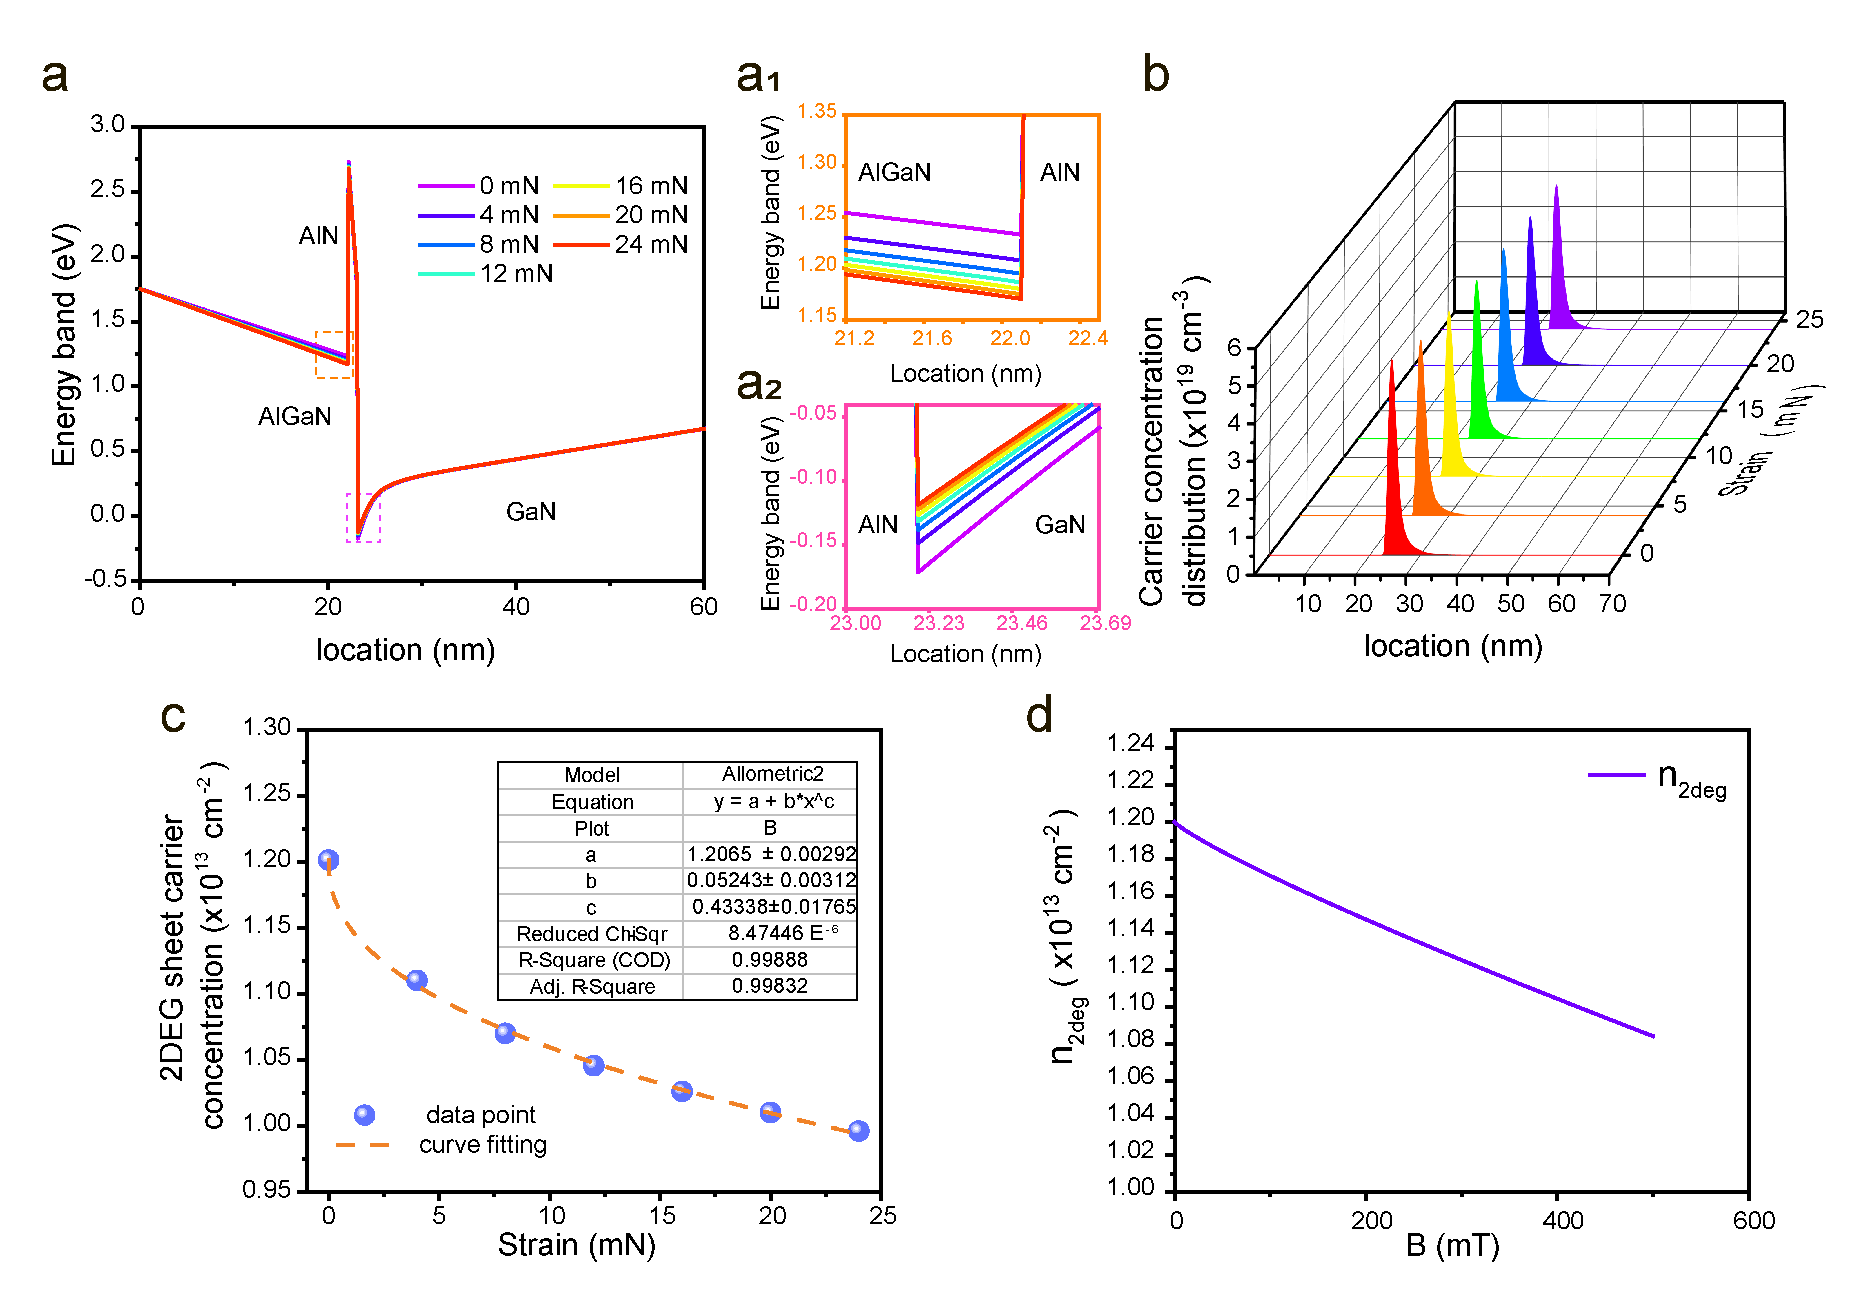
\includegraphics[width=0.9\textwidth]{ch4_7}
\caption[The calculated energy band and 2DEG concentration n AlGaN/AlN/GaN heterojunction under magnetic force in $+z$ direction.]{The calculated energy band and 2DEG concentration n AlGaN/AlN/GaN heterojunction under magnetic force in $+z$ direction. (a) The conduction band under external strains. (b) The carrier concentration distribution and the 2DEG concentration (c) under external strains, as well as the fitting curve. (d) The 2DEG concentration under magnetic force in $+z$ direction.}
\label{fig:4.7}
\end{figure}

\noindent where $\varepsilon_{0}$ is vacuum permeability with the unit \unit{\henry\per\m}, $B$ is external magnetic field with the unit \unit{\tesla}, $A_{m}$ is the area of magnetic film with the unit \unit{\square\m}. Hence, combing these two equations, we have eventually derived the linear relationship between 2DEG concentration \index{Two-dimensional electron gas (2DEG)} ($n_{2deg}$) and external magnetic field ($B$).
\begin{equation}
	n_{2deg}=1.2-0.21\times B^{0.86}
\label{eq:4.4}
\end{equation} 

The \index{Magnetosensory power MEMS devices (MPD)} curve of the \autoref{eq:4.4} is shown in \autoref{fig:4.7}d. It clearly shows that when the magnetic field \index{Magnetic!field} increases from 0 to 400 \unit{\milli\tesla}, the 2DEG \index{Two-dimensional electron gas (2DEG)} concentration decreases quasi-linearly with the external magnetic field. By virtue of semiconductor theory, the source-drain current of \index{HEMT} AlGaN/GaN HEMT is proportional to the 2DEG concentration. Therefore, we can conclude that the source-drain current and \index{Output!power} output power are quasi-linearly related to the external magnetic field.

We \index{Magnetosensory power MEMS devices (MPD)} then study the case where the normal force generated by the \index{Magnetic!field} magnetic field is in the $-z$ direction, which is exactly the experimental condition in this study. The self-consistent calculation result is displayed in \autoref{fig:4.8} and \autoref{tab:4.4}. It is clearly shown that as the strain on the cantilever \index{Cantilever} increases (from 0 to 24 \unit{\mN}), the $E_{c}$ of AlGaN is lifted upward while the Ec of GaN is lowered down, which deepen the \index{Potential!well} potential well of AlN/GaN heterojunction (\autoref{fig:4.8}a). Therefore, the \index{Carrier!concentration} carrier \index{Carrier!distribution} concentration distribution of the heterojunction is significantly increased, as shown in \autoref{fig:4.8}b. It is clearly shown that the peak value of carrier concentration increases with strain, indicating that more electrons are confined in the AlN/GaN potential well. According to the theory of semiconductor physics, the 2DEG sheet carrier concentration under different strains can be obtained by integrating the carrier concentration distribution along the c-axis, resulting in \autoref{fig:4.8}c. It illustrates that the 2DEG \index{Two-dimensional electron gas (2DEG)} sheet carrier concentration increases rapidly with external strains (over a range of 0 to 24 \unit{\mN}).

In order to further explain the quasi-linear modulation relationship of external magnetic field ($B$) to source-drain current ($I_{ds}$) and changes of output power density ($\Delta P$), we also perform a curve-fitting on the calculated 2DEG sheet carrier \index{Carrier!concentration} concentration in \autoref{fig:4.8}c. The fitting result (\autoref{tab:4.5}) shows that the 2DEG concentration is about 0.5 power of external strain in our strain range and can be expressed as
\begin{equation}
	n_{2deg}=1.2+0.04 \times F^{0.47}
\label{eq:4.}
\end{equation}
Combing the equation with the \autoref{eq:4.3}, we have eventually derived the linear relationship between 2DEG concentration ($n_{2deg}$) and external magnetic field ($B$). 
\begin{equation}
	n_{2deg}=1.2+0.168\times B^{0.94}
\label{eq:4.6} 
\end{equation}


\begin{table}[H]
\renewcommand\arraystretch{1.2}
\centering
\caption[The calculated result for $n_{2deg}$-strain relationship under the magnetic force in $-z$ direction]{The \index{Magnetosensory power MEMS devices (MPD)} calculated result for $n_{2deg}$-strain relationship under the magnetic force in $-z$ direction}
\setlength{\tabcolsep}{7mm}{
\begin{tabular}{cc}
\hline \hline
Strain (\unit{\mN}) & 2DEG Concentration ($\times 10^{13}$ \unit{\per\square\cm}) \\ \hline \hline
0           & 1.2011                          \\
4           & 1.2811                          \\
8           & 1.3196                          \\
12          & 1.3452                          \\
16          & 1.3645                           \\
20          & 1.3806                          \\
24          & 1.3941                          \\ \hline \hline
\end{tabular}}
\label{tab:4.4}
\end{table}

\begin{table}[H]
\renewcommand\arraystretch{1.2}
\centering
\caption[The fitting curve of the calculated $n_{2deg}$-strain relationships under the magnetic force in $-z$ direction]{The \index{Two-dimensional electron gas (2DEG)} fitting curve of the calculated $n_{2deg}$-strain relationships under the magnetic force in $-z$ direction}
\setlength{\tabcolsep}{12mm}{
\begin{tabular}{cc}
\hline \hline
Model           & Allometric2                    \\ \hline \hline
Equation        & $y = a + b\times x^{c}$ \\
a               & 1.2005 ± 0.00313              \\
b               & 0.04423 ±0.00315             \\
c               & 0.46889 ±0.02115              \\
Reduced Chi-Sqr & 9.7702E-6                     \\
R-Square (COD)  & 0.99856                        \\
Adj. R-Square   & 0.99784                        \\ \hline \hline
\end{tabular}
\label{tab:4.5}}
\end{table}


                                     

The curve of the \autoref{eq:4.6} is shown in \autoref{fig:4.8}d. It clearly shows that when the magnetic field \index{Magnetic!field} increases from 0 to 400 \unit{\mN}, the 2DEG \index{Two-dimensional electron gas (2DEG)} concentration increases quasi-linearly with the external magnetic field. Therefore, the source-drain current of AlGaN/GaN HEMT \index{HEMT} is proportional to the 2DEG concentration and we can conclude that the source-drain current and \index{Output!power} output power are quasi-linearly related to the external magnetic field. The theoretical model agrees well with the experimental result.

The 2DEG sheet carrier concentration \index{Carrier!concentration} when the MPD rotates at different angles under 0-400 \unit{\milli\tesla} magnetic fields have also been further simulated to imitate the mechanism that birds orient themselves by sensing the angle and magnitude of the geomagnetic field. The formula under the magnetic force in the $+z$ direction and $-z$ direction are derived in \autoref{eq:4.7} and \autoref{eq:4.8}, respectively.
\begin{equation}
	n_{2deg}=1.2-0.21\times B^{0.86}\times cos \left( \frac{(\theta -180)\pi}{180} \right)
\label{eq:4.7}
\end{equation}
\begin{equation}
	n_{2deg}=1.2+0.168\times B^{0.94}\times cos \left( \frac{\theta\pi}{180} \right)
\label{eq:4.8}
\end{equation}
where $\theta$ is the rotation angle.

The \index{Magnetosensory power MEMS devices (MPD)} curve has been shown in \autoref{fig:4.8}e. It clearly illustrates that the 2DEG concentration \index{Two-dimensional electron gas (2DEG)} of MPD has an approximately sinusoidal relationship with the rotation angle, and its maximum value increases significantly with the increase of the magnetic field. Therefore, it can be concluded that the output current and power of MPD show a sinusoidal relationship with the angle of the magnetic field, and a linear relationship with the magnitude of the magnetic field when sensing different external magnetic fields. This indicates that the output current and power of MPD can be effectively modulated by the angle and magnitude of the magnetic field, showing excellent orientation and sensing capabilities.


\begin{figure}[H] 
\centering    
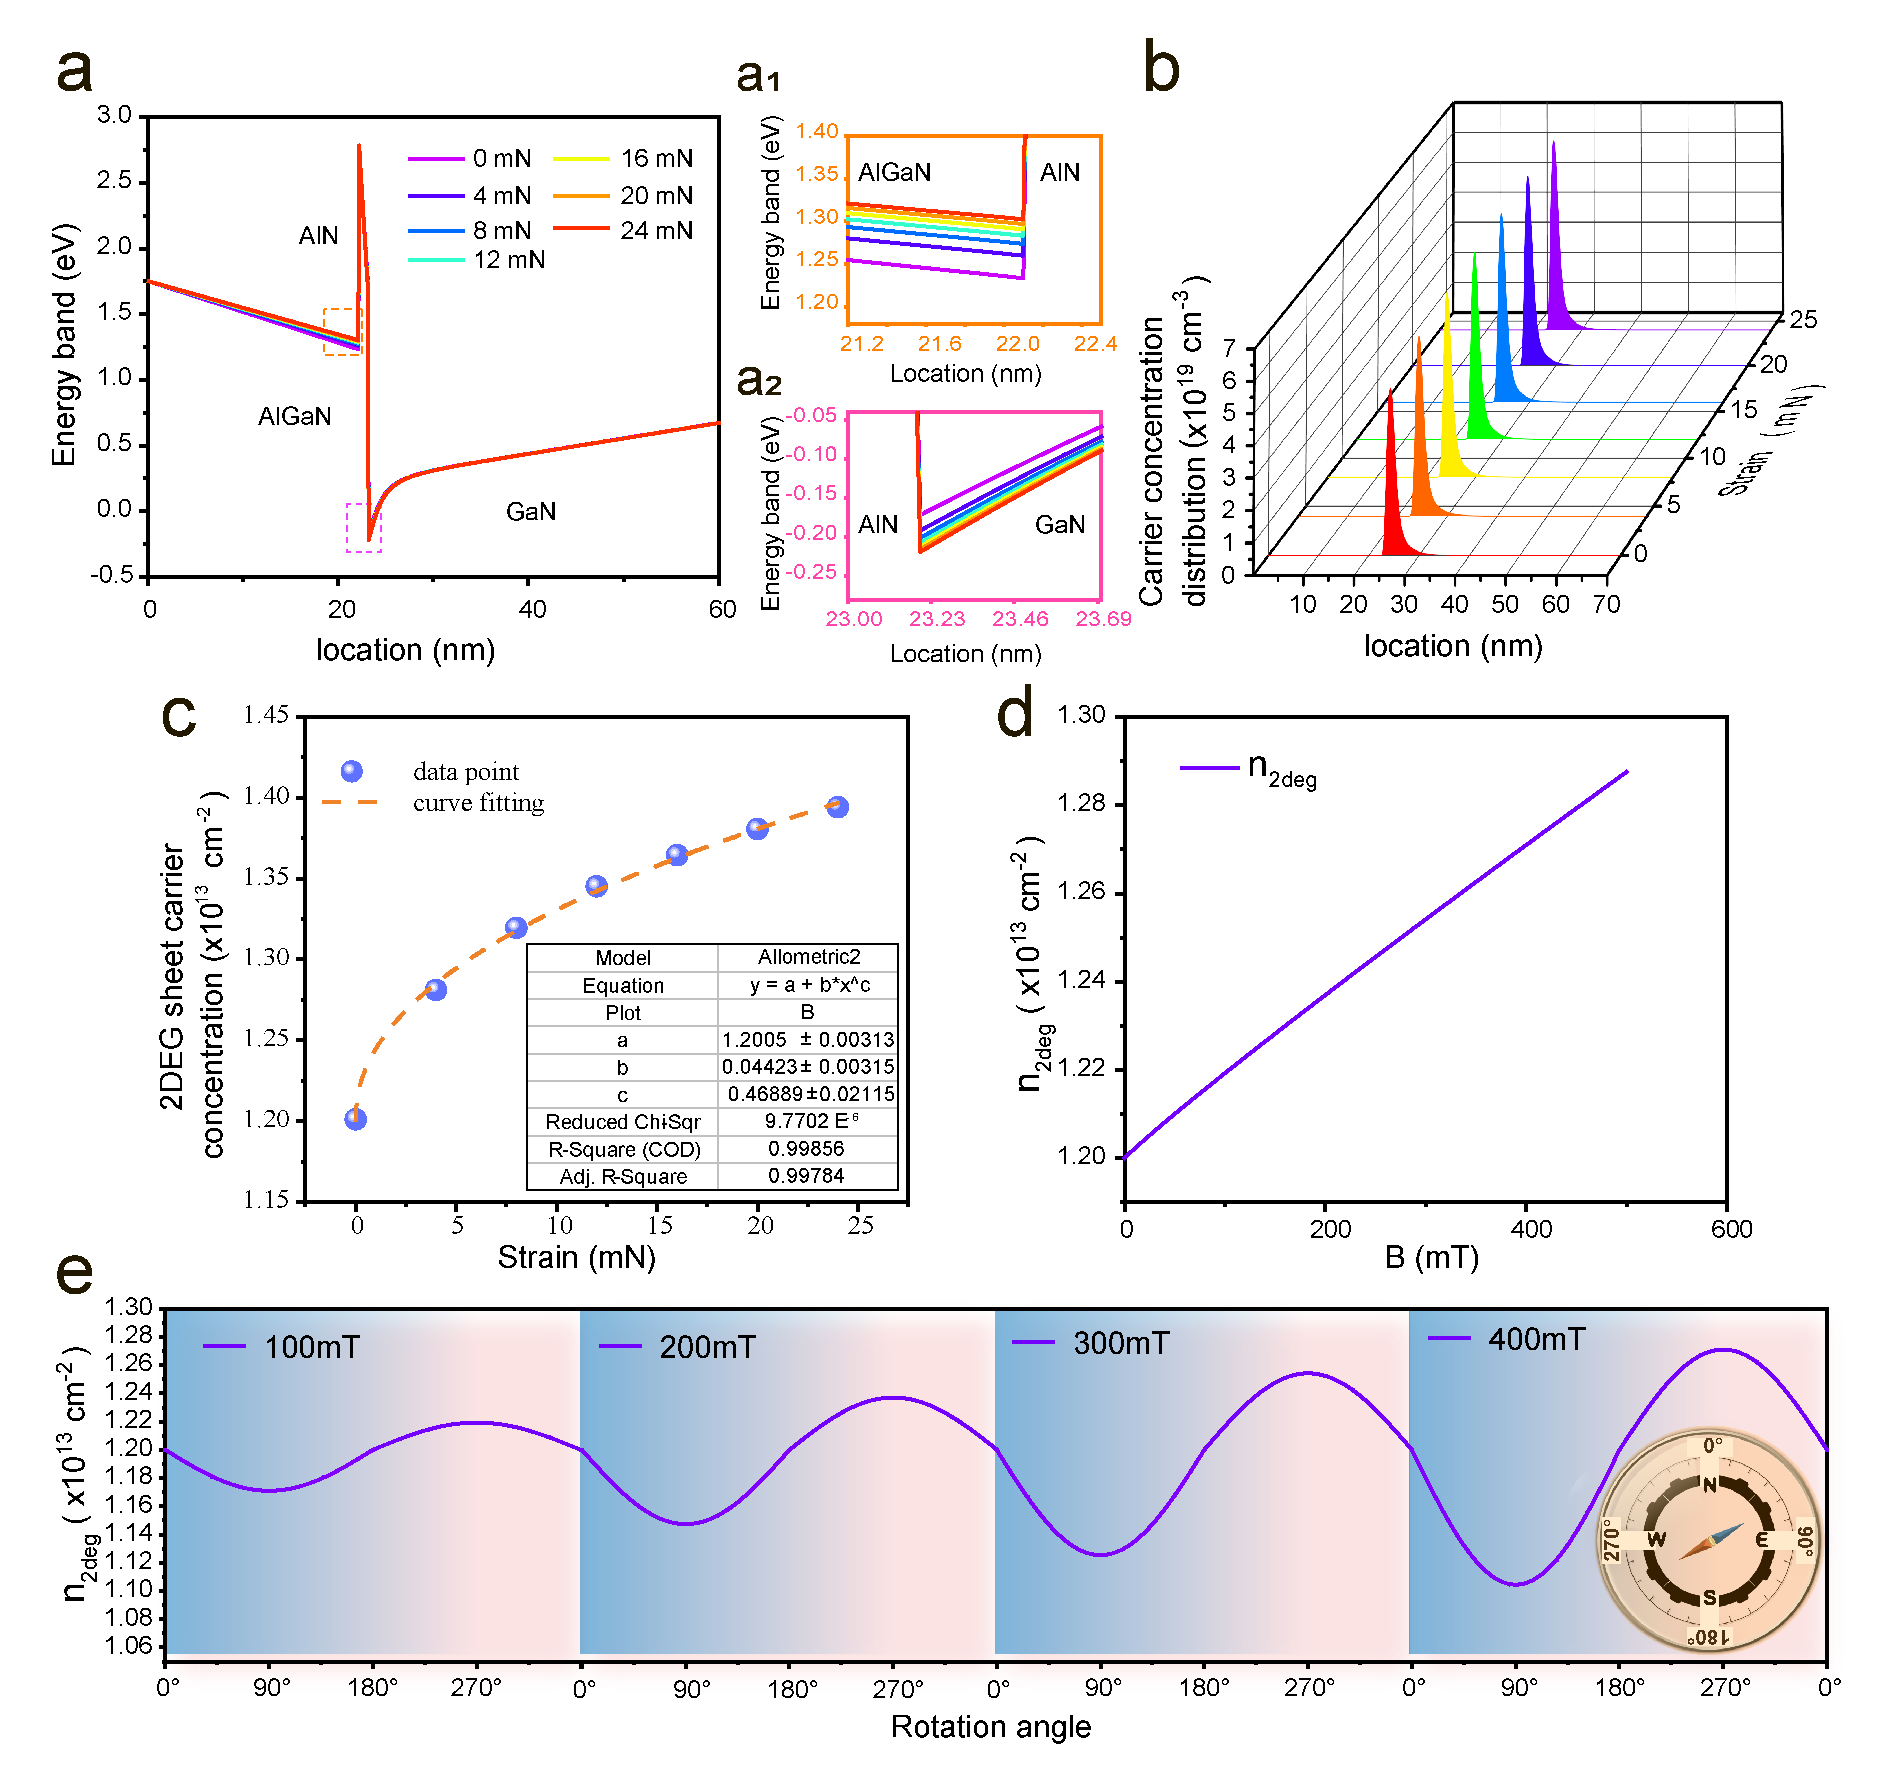
\includegraphics[width=0.9\textwidth]{ch4_8}
\caption[The calculated energy band and 2DEG concentration in AlGaN/AlN/GaN heterojunction under magnetic force in $-z$ direction and rotation.]{The calculated energy band and 2DEG concentration in AlGaN/AlN/GaN heterojunction under magnetic force in $-z$ direction and rotation. (a) The conduction band under external strain. (b) The carrier concentration distribution and the 2DEG concentration (c) under external strains, as well as the fitting curve. (d) The 2DEG concentration under magnetic force in $-z$ direction. (e) The 2DEG concentration of SPD at different rotation angles under 0 $\sim$ 400 \unit{\milli\tesla} magnetic fields.}
\label{fig:4.8}
\end{figure}



\section{Summary}
In \index{Magnetosensory power MEMS devices (MPD)} summary, we demonstrate a magnetosensory power device that can utilize external magnetic field to modulate the output power of the device by the emulation of magnetoreception in nature. Based on the piezotronic effect, the strain-induced piezoelectric polarization charges can modify the energy band profile of the local AlGaN/AlN/GaN heterojunction, and effectively adjust the 2DEG concentration to tune/control the output power of the MPD. Due to the design of the magnetic cantilever \index{Cantilever} of the MPD, the external magnetic field can introduce a normal compressive strain at the front end of the \index{Cantilever} cantilever, thereby triggering piezotronics effect. Under the action of the external magnetic field of 0 $\sim$ 400 \unit{\milli\tesla}, when the gate voltage is -5 \unit{\V}, the saturation output power density of MPD increases quasi-linearly from 18.04 \unit{\W\per\square\mm} to 18.94 \unit{\W\per\square\mm}, showing good magnetic field-power modulation characteristics. Meanwhile, the gate voltage of MPD can control the working point of the output power in a larger range. The maximum output power density of MPD can reach 85.8 \unit{\W\per\square\mm} at 1 \unit{\V} gate voltage under 200 \unit{\milli\tesla} magnetic field, thereby realizing the two-dimensional control of the output power by the external magnetic field and the gate \index{Voltage!gate voltage} voltage. This work not only provides insights into interactive electronics \index{Interactive electronic} that integrate sensing and control functionalities, but also promotes the development of bionic AI smart devices, especially in applications of very large scale integration (VLSI) systems that mimic neurobiological architectures present in the nervous \index{Magnetosensory power MEMS devices (MPD)} system \cite{mead1990neuromorphic,furber2016large}.

\nomenclature{$\theta$}{Rotation angle}
\nomenclature{$n_{2DEG}$}{2DEG concentration}
\nomenclature{$B$}{External magnetic field}
\nomenclature{$A_{m}$}{Area of magnetic film}

\nomenclature[z-MPD]{MPD}{Magnetosensory power device}
 
 